%-- einleitung
\section{Konzept}

\subsection{Anforderungsanalyse}

\begin{table}[H]
\caption{Funktionale Anforderungen}
\begin{tabular}{|c|p{12cm}|}
Nummer & Beschreibung \\
\hline
1FA & Die Liste der Städte (Namen + Distanzen) sollen aus einer Datei (mit bestimmter Formatierung) auslesbar sein, damit diese Daten ohne Programmieraufwand verändert werden können. \\  
2FA & Das System soll mit Genetischen Algorithmen das Travelling Salesman Problem umsetzen. \\  
3FA & Das System soll Routen auf Grundlage derer Gesamtdistanz beurteilen und weiterverarbeiten. \\  
\end{tabular}
\label{tab:fa}
\end{table}

\begin{table}[H]
\caption{Nichtfunktionale Anforderungen}
\begin{tabular}{|c|p{10cm}|}
 Nummer & Beschreibung \\ 
\hline
1NFA & Das System soll auf Windows 10 ausführbar sein.\\
2NFA & Das System soll vollständig dokumentiert sein.\\
3NFA & Das System soll leicht testbar sein.\\
4NFA & Das System soll leicht bedienbar sein.\\
5NFA & Das System soll als Executable ausführbar sein.\\
\end{tabular}
\label{tab:nfa}
\end{table}

\subsection{Systemmodellierung}

\begin{figure}[H]
\centering
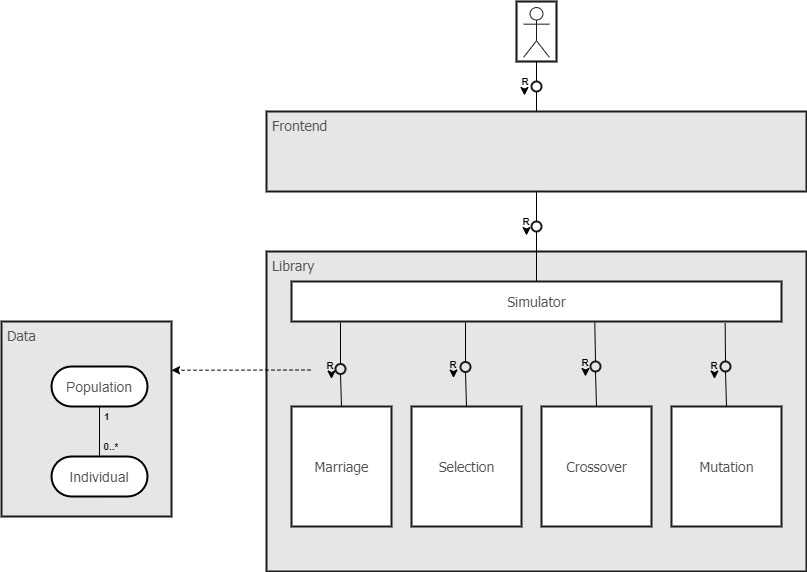
\includegraphics[width=1\textwidth]{img/Vortrag/Systemmodellierung.png}
\caption{Systemmodellierung}
\label{fig:systemmodellierung}
\end{figure}

%--